This section explains and motivates the method used for the experiment conducted in this thesis. First, we provide a summary of the overall procedure to give a broad understanding without delving into specific details. Then, each component is described in detail in its own subsection.

% \begin{generalinstructions}
% \begin{compactenum}
% \item Method overview
% \item Test of marginal model (Does it deviate for different distributions?)
% \item Choice of method for copula
% \item Portfolio testing (Main experiment)
% \end{compactenum}
% \end{generalinstructions}

%%%%%%%%%%%%%%%%%%%%%%%%%%%%%%%%%%%%%%%%%%%%%%%%%%%%%%%%%%%%%%%%%%%%%%%%%%%%%%%
%%%% Method overview
%%%%%%%%%%%%%%%%%%%%%%%%%%%%%%%%%%%%%%%%%%%%%%%%%%%%%%%%%%%%%%%%%%%%%%%%%%%%%%%
\subsection{Method overview}
This section describes the methodology used in the experiment, which is divided into three main components corresponding to the different research questions.

\RQone was investigated by testing how well the marginal distributions are fitted by the marginal model. The aim is to verify whether the fitted marginal distribution aligns with the true distribution of the data. Theoretically, there should be no difference between the fitted and the true marginal distribution, given a sufficiently large sample. This validation is crucial because copulas are invariant under strictly increasing transformations, implying that the fitted copula should accurately replicate the joint distribution regardless of the specific marginal distributions used. In the main experiment, it is known that log returns are normally distributed. However, since this is not always the case in reality, we want to test how well the \gls{NC} marginal models perform under different conditions.

The second part of the method addresses \RQtwo and involves testing which hyperparameter values allow the copula model to train effectively. This is done by training several models with varying hyperparameter settings and selecting those that minimize the loss function. The goal is to identify parameter configurations that consistently produce valid copulas using the \gls{NC} across different datasets. This ensures robustness and general applicability of the training scheme.

The third component constitutes the main experiment and aims to answer \RQthree. The overall procedure is as follows: portfolios with various dependency structures are generated by sampling data in probability space from different copulas and transforming it to return space using the \gls{ITM}, yielding dependent, normally distributed returns (as described in \Cref{sec:CopulaUseCase}). This ensures that the generated portfolios have normal marginal distributions, eliminating the need to fit them in this experiment. This setup enables a focused evaluation of the copula's performance, isolated from potential marginal fitting errors.

The generated normal random variables are then used as shocks in the Weiner process when simulating a \gls{GBM} using the Euler-Maruyama scheme, resulting in realistic stock price time series suitable for copula-based analysis.

These simulated price series are divided into two segments: historical and future returns. This division is illustrated in \Cref{fig:DataDivision}, where blue and orange lines represent different simulated stocks. The dashed black line denotes the division point, with the fitting part used to fit the copulas and the testing part treated as the ground truth for future returns. As discussed in \Cref{sec:MonteCarlo}, a key assumption in \gls{MC} methods is that the statistical distribution of the data remains constant over time. Random numbers sampled from the fitted copula should thus mimic the joint distribution if the copula accurately captures dependency. This is the core aim of the thesis: to evaluate how well various copulas can replicate the data’s joint distribution.

\begin{figure}
\centering
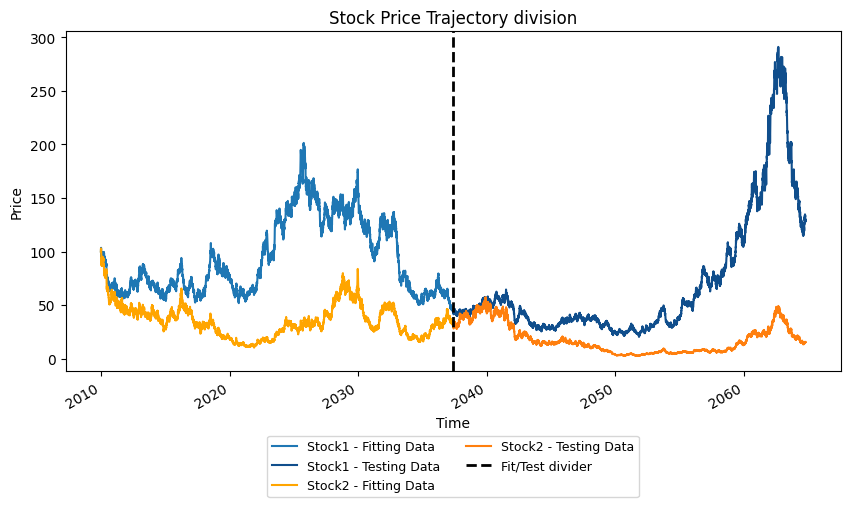
\includegraphics[width=0.8\textwidth]{4Method/pictures/DataDivision.png}
\caption{Illustration of how the data is divided into fitting and testing parts.}
\label{fig:DataDivision}
\end{figure}

An example comparison between the test data and data generated from a fitted copula is shown in \Cref{fig:TestSampleComparison}. The red points represent test data from a Clayton copula, while the blue points are samples from a Gaussian copula fitted to the corresponding fitting data. If the copula successfully captures dependency, the two distributions should be visually and statistically similar.

\begin{figure}
\centering
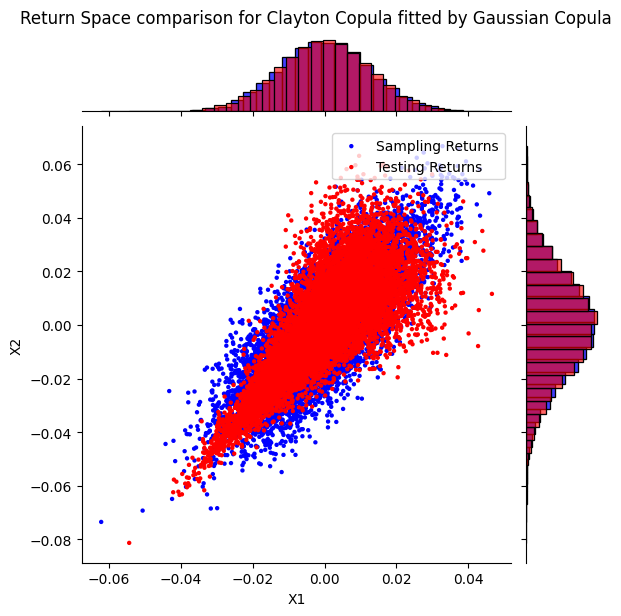
\includegraphics[width=0.5\textwidth]{4Method/pictures/TestSampleComparison.png}
\caption{Comparison between test data and data sampled from a fitted copula.}
\label{fig:TestSampleComparison}
\end{figure}

To evaluate the copulas’ ability to model dependency accurately, it is necessary to compare the generated and test datasets. Simulated data is used to ensure that the joint distribution remains stationary, satisfying the \gls{MC} assumption. If the copula-generated data closely resembles the test data, the dependency is well captured. Otherwise, it indicates the copula’s limitations.

It is important to emphasize that the core assumption behind using copulas for \gls{MC} simulation is that the joint distribution observed historically remains valid into the future.

To quantify the similarity between test and sampled data, the distance metric described in \Cref{sec:GoodnessOfFit} is used. This allows for calculating an average distance for each copula over multiple datasets and identifying the best-performing copula overall.

%%%%%%%%%%%%%%%%%%%%%%%%%%%%%%%%%%%%%%%%%%%%%%%%%%%%%%%%%%%%%%%%%%%%%%%%%%%%%
%%%% Marginal model test
%%%%%%%%%%%%%%%%%%%%%%%%%%%%%%%%%%%%%%%%%%%%%%%%%%%%%%%%%%%%%%%%%%%%%%%%%%%%%
\subsection{Marginal model test}
To validate the marginal model, a test is conducted to assess how closely the fitted marginal distribution matches the true distribution. This is done by generating data from known distributions and fitting the marginal model to it. The data is then transformed into probability space using the \gls{PIT}, both with the fitted and true distributions. A QQ-plot is generated to visualize the similarity between the fitted and true distributions. 

Note that the generated data is subject to random noise, so the observed distribution may differ slightly from the true distribution, even though they are theoretically identical. Nevertheless, this test offers a good benchmark for how accurately the model fits marginals, providing a reference for what might be used if a \gls{NN} were not employed.

The tested distributions, along with their parameter values and descriptions, are shown in \Cref{tab:distributions}. For this test, all terms in the loss function defined in \Cref{sec:NeuralCopulaLoss} are equally weighted. Each distribution is tested using 10,000 data points.

\begin{table}[h]
    \centering
    \caption{Distributions and parameters used for the marginal model test.}
    \begin{tabular}{@{}ccl@{}}
        Distribution & Parameters & Description \\
        \toprule
        Gaussian & $\mu=0, \sigma=1$ & Standard normal distribution \\ 
        Student's $t$ & $\nu=5$ & Student's $t$-distribution with 5 degrees of freedom \\ 
        Uniform & $a=0, b=1$ & Uniform distribution on [0, 1] \\ 
        Exponential & $\lambda=1$ & Exponential distribution with rate 1 \\ 
        Laplace & $\mu=0, b=1$ & Laplace distribution with mean 0 and scale 1 \\ 
        Log-normal & $\mu=0, \sigma^2=1$ & Log-normal distribution with mean 0 and variance 1 \\ 
    \end{tabular}
    \label{tab:distributions}
\end{table}


%%%%%%%%%%%%%%%%%%%%%%%%%%%%%%%%%%%%%%%%%%%%%%%%%%%%%%%%%%%%%%%%%%%%%%%%%%%%%
%%%% Neural copula testing
%%%%%%%%%%%%%%%%%%%%%%%%%%%%%%%%%%%%%%%%%%%%%%%%%%%%%%%%%%%%%%%%%%%%%%%%%%%%%
\subsection{Neural Copula training scheme test}
This section outlines the procedure for identifying the best hyperparameters that produce a valid copula function. A copula is considered valid if it satisfies the conditions defined in \Cref{def:copula}. For the \gls{NC}, this means that all loss terms—except the first—defined in \Cref{sec:NeuralCopulaLoss}, should approach zero after training.

To ensure robustness across datasets, the model will be tested on several datasets. For each dataset, a grid of hyperparameter values will be evaluated. These include solver type, learning rate, number of epochs, batch size, network architecture, and learning rate scheduler. This results in a large number of parameter combinations designed to identify a universally effective training setup. To keep runtime feasible, the grid is limited to 288\todo{Change} combinations, tested across five datasets using a computing cluster.

The datasets used for testing are listed in \Cref{tab:DatasetsTestedOn}, which specifies the copula, its parameters, and a dataset name for reference. The hyperparameter grid is summarized in \Cref{tab:se_hyperparams}. Parameters like "Network layers" and "Network neurons" define the \gls{NN} architecture, while "Learning rate", "Scheduler", and "Solver" relate to the optimization process. "Epochs" and "Batch size" govern training duration and granularity.

\begin{table}[h!]
    \centering
    \caption{Datasets used to test the \gls{NC} hyper parameters and loss function weights.}
    \begin{tabular}{lll}
    \textbf{Copula} & \textbf{Parameter} & \textbf{Name}  \\
    \hline
    Gaussian & $\rho:0$ & Independece \\
    Gaussian & $\rho:0.7$ & Positive Dependece \\
    Gaussian & $\rho:-0.7$ & Negative Dependece  \\
    Gaussian & $\rho:0.999$ & Frechet Upper \\
    Gaussian & $\rho:-0.999$ & Frechet Lower \\
    \end{tabular}
    \label{tab:DatasetsTestedOn}
\end{table}

\begin{table}[h!]
    \centering
    \caption{Hyperparameter grid choices the test of the \gls{NC} fitting procedure.}
    \begin{tabular}{ll}
    \textbf{Hyperparameter} & \textbf{Options} \\
    \hline
    Network layers & 2, 3, 4 \\
    Network neurons & 5, 10 \\
    Learning rate & 0.1, 0.01 \\
    Scheduler & step, exponential, None \\
    Solver & ADAM, SGD \\
    Epochs & 10000, 5000 \\
    Batch size & 1024, 2048 (Remove batch size) \\
    \end{tabular}
    \label{tab:se_hyperparams}
\end{table}

% Each hyperparameter combination is evaluated using an ensemble of 10 runs to mitigate variability due to random initialization. The best run from each ensemble is selected for evaluation.

After testing all combinations, the best-performing setup across all datasets—measured by average loss—will be selected. If constraint-related loss terms are close to zero, the copula is considered valid. This best model is then used in the final experiment described in \Cref{sec:PortfolioTesting}.

Additionally, the effect of varying the weights of different loss function terms, defined in \Cref{sec:NeuralCopulaLoss}, will be examined. While the first term is fixed to one, linear combination weights of 0.5, 1, and 2, are tested for each of the other loss terms. The goal is to determine if emphasizing certain terms improves performance. This test uses the previously selected best hyperparameters, and evaluation is based on the equally weighted loss for fair comparison. Each copula from the hyperparameter test is included in this analysis to assess the effect of loss term weighting.


%%%%%%%%%%%%%%%%%%%%%%%%%%%%%%%%%%%%%%%%%%%%%%%%%%%%%%%%%%%%%%%%%%%%%%%%%%%%%%
%%%% Portfolio testing
%%%%%%%%%%%%%%%%%%%%%%%%%%%%%%%%%%%%%%%%%%%%%%%%%%%%%%%%%%%%%%%%%%%%%%%%%%%%%%
\subsection{Portfolio Testing}\label{sec:PortfolioTesting}
This section outlines the methodology used to evaluate copula models on synthetic financial portfolios with controlled dependence structures.

\subsubsection{Data Generation}
To assess the performance of different copulas, synthetic test portfolios of stock price data are generated. The aim is to isolate the role of the copula by ensuring consistent and known marginal distributions across all datasets, thereby preventing confounding effects from the marginal fitting process. As copulas are invariant under strictly increasing transformations (see \Cref{the:TranslationInvariance}), the choice of marginal distribution is arbitrary. In this study, standard normal distributions are used for all marginals.

Dependence is introduced via analytical copulas with varying parameters. Data is first sampled in probability space from the specified copulas. These samples are then transformed using the inverse CDF of the standard normal distribution, producing dependent samples with standard normal marginals. These samples are subsequently used as random shocks in simulating bivariate Geometric Brownian Motion (GBM) via the Euler-Maruyama scheme described in \Cref{sec:EulerMaruyama}.

This process yields synthetic price trajectories that reflect realistic financial behavior while preserving the controlled dependence introduced by the copula. The copulas and corresponding parameters used in the data generation process are summarized in \Cref{tab:DatasetsUsed}. Each simulation runs for 10,000 time steps (interpreted as trading days), with both assets having a drift of 0.03 and volatilities of 0.2 and 0.3, respectively.

\begin{table}[h!]
    \centering
    \caption{Portfolios used to evaluate the different copulas.}
    \begin{tabular}{ll}
    \textbf{Copula} & \textbf{Parameters} \\
    \hline
    Gaussian & Correlation: 0 \\
    Gaussian & Correlation: 0.7\\
    Student's $t$ & $\rho$: -0.8, $\nu$: 3\\
    Clayton & $\alpha$: 4 \\
    \end{tabular}
    \label{tab:DatasetsUsed}
\end{table}

The resulting datasets are visualized in \Cref{fig:DatasetsUsed}, which shows both the simulated price trajectories (left) and the log returns (right). Log returns are computed and partitioned into fitting (training) and testing datasets. The blue points represent fitting data used for model estimation, while the red points denote testing data used for performance evaluation. This mirrors a real-world setting where models are trained on historical data and evaluated on future, unseen data.

\begin{figure}
    \centering
    % --- (a) Independence ---
    \begin{minipage}{0.9\textwidth}
        \centering
        \begin{minipage}{0.54\textwidth}
            \centering
            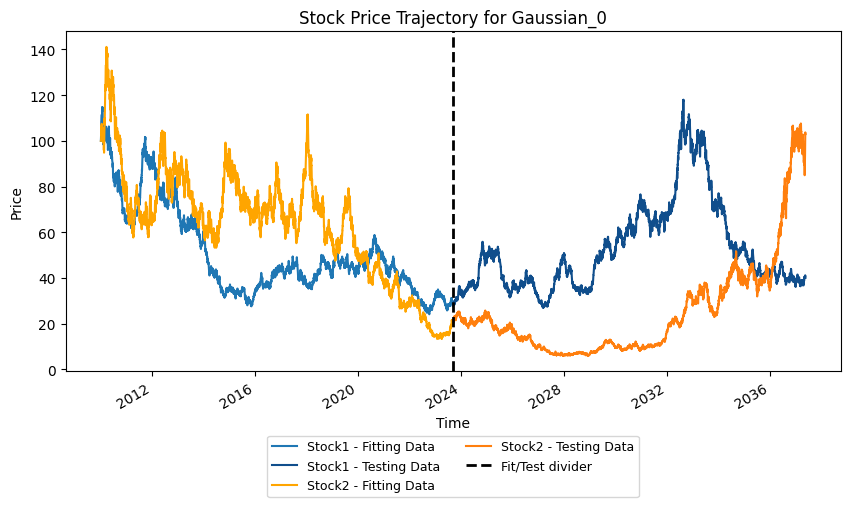
\includegraphics[width=\textwidth]{4Method/pictures/PricesGaussian_0.png}
        \end{minipage}
        \hfill
        \begin{minipage}{0.34\textwidth}
            \centering
            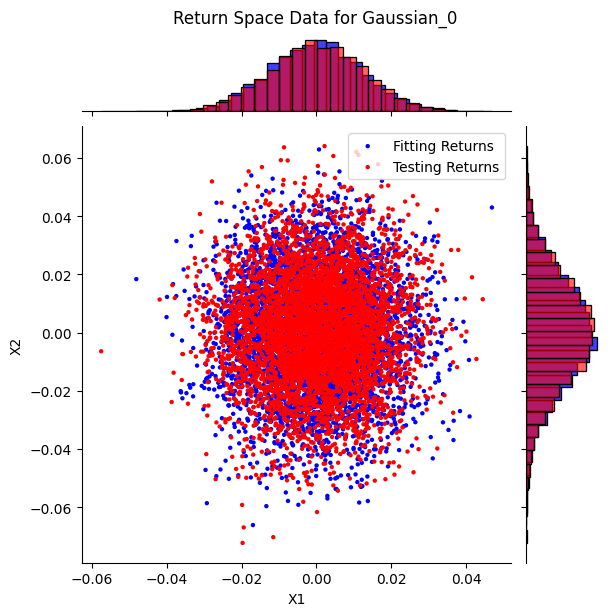
\includegraphics[width=\textwidth]{4Method/pictures/ReturnsGaussian_0.png}
        \end{minipage}
        \subcaption*{(a) Gaussian (independent)}
    \end{minipage}
    \hfill
    % --- (b) Student's t ---
    \begin{minipage}{0.9\textwidth}
        \centering
        \begin{minipage}{0.54\textwidth}
            \centering
            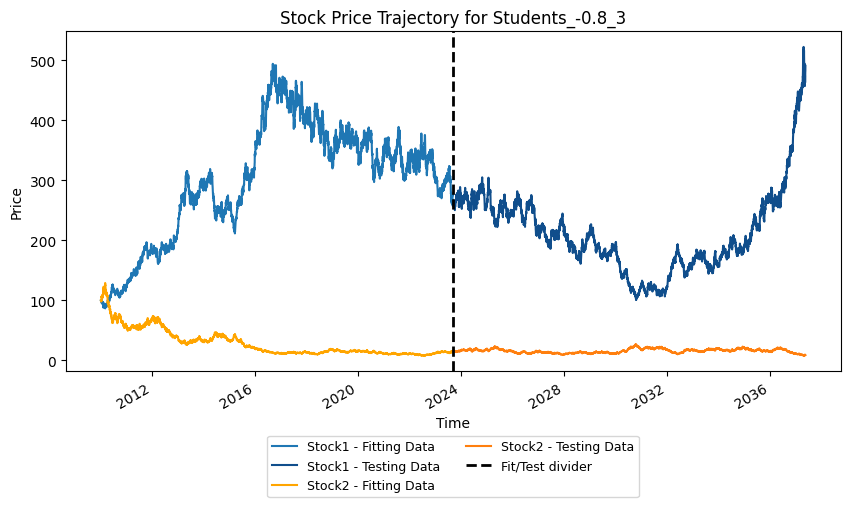
\includegraphics[width=\textwidth]{4Method/pictures/PricesStudents_-08_3.png}
        \end{minipage}
        \hfill
        \begin{minipage}{0.34\textwidth}
            \centering
            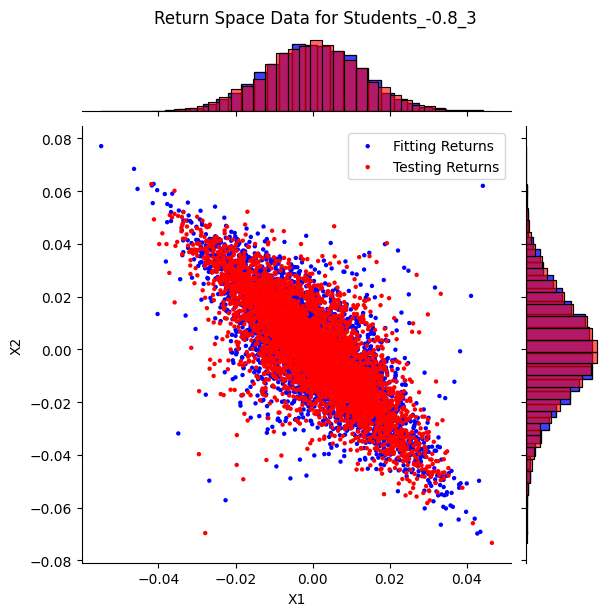
\includegraphics[width=\textwidth]{4Method/pictures/ReturnsStudents_-08_3.png}
        \end{minipage}
        \subcaption*{(b) Student's $t$ ($\rho = -0.8$, $\nu = 3$)}
    \end{minipage}
    \vfill
    % --- (c) Gaussian 0.7 ---
    \begin{minipage}{0.9\textwidth}
        \centering
        \begin{minipage}{0.54\textwidth}
            \centering
            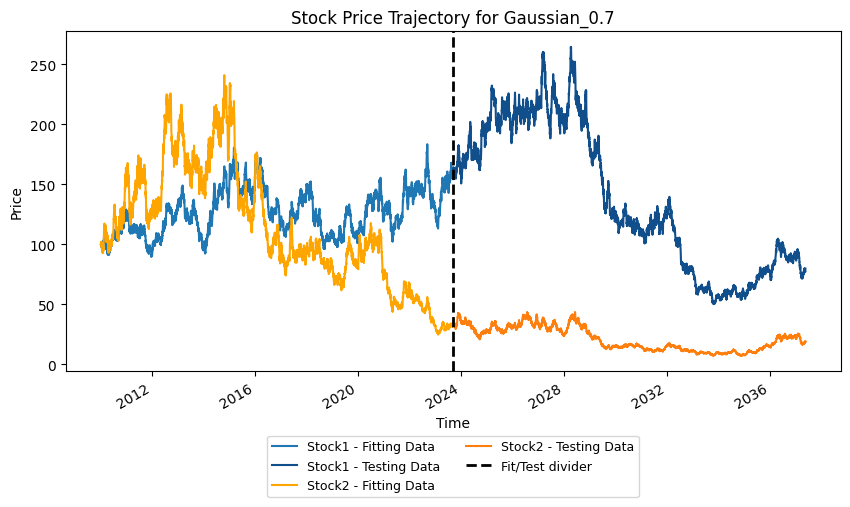
\includegraphics[width=\textwidth]{4Method/pictures/PricesGaussian_07.png}
        \end{minipage}
        \hfill
        \begin{minipage}{0.34\textwidth}
            \centering
            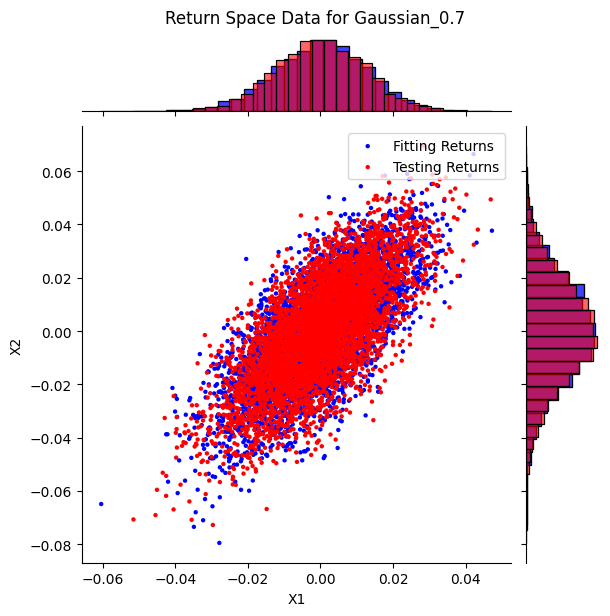
\includegraphics[width=\textwidth]{4Method/pictures/ReturnsGaussian_07.png}
        \end{minipage}
        \subcaption*{(c) Gaussian ($\rho = 0.7$)}
    \end{minipage}
    \hfill
    % --- (d) Clayton ---
    \begin{minipage}{0.9\textwidth}
        \centering
        \begin{minipage}{0.54\textwidth}
            \centering
            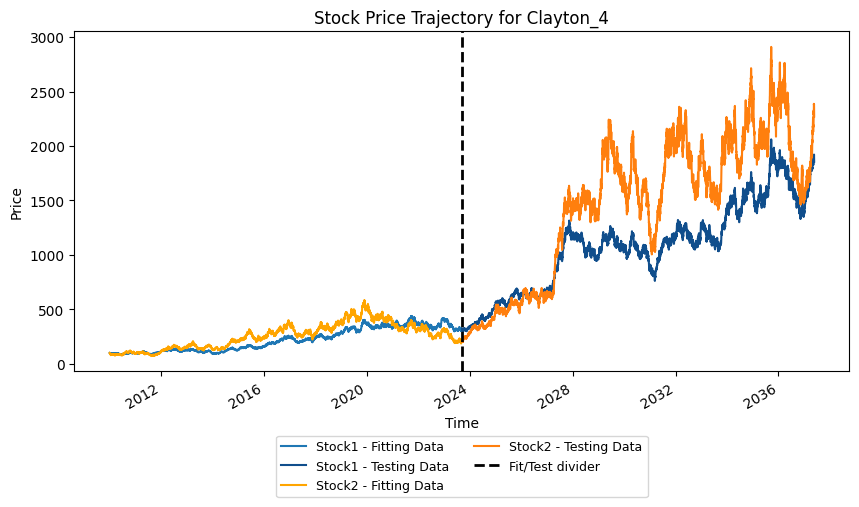
\includegraphics[width=\textwidth]{4Method/pictures/PricesClayton_4.png}
        \end{minipage}
        \hfill
        \begin{minipage}{0.34\textwidth}
            \centering
            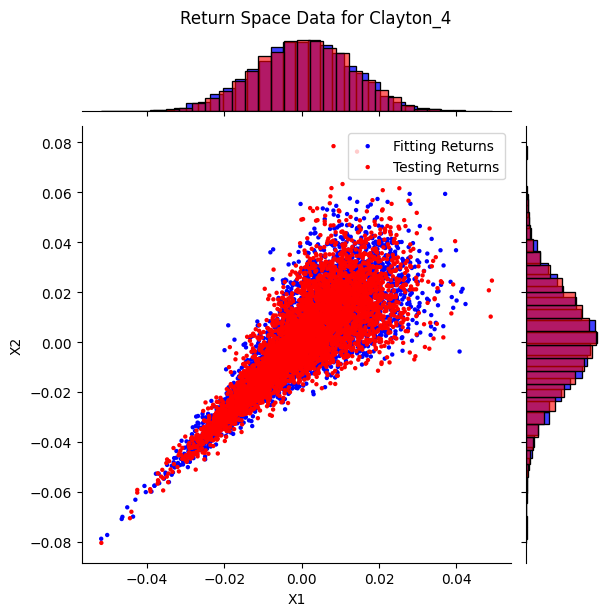
\includegraphics[width=\textwidth]{4Method/pictures/ReturnsClayton_4.png}
        \end{minipage}
        \subcaption*{(d) Clayton ($\alpha = 4$)}
    \end{minipage}
    \caption{Simulated test portfolios: Price trajectories (left) and corresponding log returns (right). Blue = fitting data, Red = testing data.}
    \label{fig:DatasetsUsed}
\end{figure}

\subsubsection{Model Fitting}
The log returns from the fitting portion of each dataset are first standardized to zero mean and unit variance. These normalized returns are then used to estimate the copula parameters. Fitting procedures follow the methods outlined in \Cref{sec:GaussianCopula} for the Gaussian copula, \Cref{sec:StudentsCopula} for the Student's $t$ copula, \Cref{sec:ClaytonCopula} for the Clayton copula, and \Cref{sec:NeuralCopulaFittingAndSampling} for the \gls{NC}.


\subsubsection{Model Sampling}
A key use case for copulas is generating dependent samples for Monte Carlo simulations \citep[p.~40]{Nelsen2006}. Once fitted, each copula is used to sample new data in probability space. These samples are then mapped through the inverse normal CDF and scaled to match the empirical standard deviation of the original (fitting) data.

The neural copula, unlike the others, incorporates inverse marginal models directly and does not rely on the inverse normal transformation. If the copula accurately captures the dependence structure, the resulting synthetic data should closely resemble the testing dataset.

\subsubsection{Model Evaluation}
To evaluate performance, the sampled data from each fitted copula is compared to the corresponding testing data using the distance measure described in \Cref{sec:GoodnessOfFit}. For each copula, this distance is averaged across all datasets to yield an overall performance score. This facilitates a robust comparison of model quality across varying dependence structures.

% \begin{generalinstructions}
%     \begin{compactenum}
%         \item Data Generation
%         \begin{compactenum}
%             \item Sample from copulas in probability space.
%             \item Transform samples to standard normals.
%             \item Use as random shocks in GBM simulations.
%             \item Compute log returns and split into training/testing sets.
%         \end{compactenum}
%         \item Model Fitting (for each copula).
%         \item Model Evaluation
%         \begin{compactenum}
%             \item Generate samples from each fitted copula.
%             \item Compare to test data using distribution-based distance measures.
%         \end{compactenum}
%     \end{compactenum}
% \end{generalinstructions}































%%%%%%%%%%%%%%%%%%%%%%%%%%%%%%%%%%%%%%%%%%%%%%%
%% Method before fixing using GPT
%%%%%%%%%%%%%%%%%%%%%%%%%%%%%%%%%%%%%%%%%%%%%%%

% This section explains and motivates the method used for the experiment tested in this thesis. First, we provide a summary of the method used, as this will help to give the overall procedure without getting stuck in the details. Then, a detailed description of each different part will be given in separate sections. 

% \begin{generalinstructions}
%     \begin{compactenum}
%         \item Method overview
%         \item Test of marginal model (does it deviate for some different distributions)
%         \item Choice of method for copula
%         \item Portfolio testing (Actual experiment)
%     \end{compactenum}
% \end{generalinstructions}


% %%%%%%%%%%%%%%%%%%%%%%%%%%%%%%%%%%%%%%%%%%%%%%%%%%%%%%%%%%%%%%%%%%%%%%%%%%%%%%%
% %%%% Method overview
% %%%%%%%%%%%%%%%%%%%%%%%%%%%%%%%%%%%%%%%%%%%%%%%%%%%%%%%%%%%%%%%%%%%%%%%%%%%%%%%
% \subsection{Method overview}
% This section describes the method used for the experiment. The method is divided into three main parts reflecting the different research questions. 

% \RQone was investigated by using a test of the marginal model is performed to see how well the marginal distributions are fitted. This is to see if the marginal distribution fitted by the marginal model works as intended. Theoretically there should not be any difference between the fitted marginal distribution and the true distribution of the data  given a sufficient number of samples. This is important as the copula is invariant to strictly increasing transformations, meaning that the fitted copula should be able to replicate the joint distribution of the data regardless of the marginal distributions used. In the main experiment we will know that the log returns are normally distributed. In reality this is not always the case, and therefore we want to test how well the \gls{NC} marginals works.

% The second part of the method investigates \RQtwo and consist of a test of what hyperparameter values makes the copula train the best. This is done by training several models with different hyperparameter values and choosing the parameters that result in the smallest loss. The goal of this part is to find parameter options works universally for the \gls{NC} meaning that the trained copula model produces a valid copula function that fits the data well. To do this the copulas will be trained on several different datasets to find make sure that the method works well regardless of the data. 

% The third part of the method is the main experiment that will answer \RQthree of this thesis and the overall procedure is as follows. To begin with, different portfolios with different types of dependency structures will be generated. This will be done by sampling data in probability space from different copulas and transforming it to return space using the \gls{ITM} to obtain dependent normally distributed returns, as described in \Cref{sec:CopulaUseCase}. This ensures that the marginal distributions of the created portfolios have normal marginal distributions, removing the need for fitting them in this experiment. This allows for an evaluation of the pure performance of the copula, without conflating it with potential errors from fitting marginal distributions. The generated normally distributed random numbers are then used as the random shocks from the Weiner process when simulating the \gls{GBM} using the Euler-Maruyama scheme to replicate stock price time series. This creates a realistic setting for when using copulas would be suitable.  

% The generated price time series are then divided into two different parts. These different parts represent the historical and the future returns of the portfolios. The splitting of data is illustrated in \Cref{fig:DataDivision} where the blue and orange lines are different simulated stocks over time. The price time series are divided at the dashed black line to create what we will call the fitting and testing parts. The fitting part is used for fitting the different copulas using historically observed data, the testing part can be considered the true distribution of future returns. As described when introducing \gls{MC} methods in \Cref{sec:MonteCarlo}, the key assumption is that of the statistical distribution of the data and that the distribution remains the same in the future. Hence the fitting part is used to fit the copulas to the historical data. From the fitted copula random numbers replicating the joint distribution is generated. If the copula adequately captures the dependence the generated data from the fitted copula should be similar to the future data. This is the main goal of this thesis, to evaluate how well different copulas can replicate the joint distribution of the data. An example of the what the different distributions can look like for the test data compared to the data sampled from the fitted copula can be viewed in \Cref{fig:TestSampleComparison} where the red data is the testing data from a Clayton copula that is to be replicated and the blue data is the data sampled from the fitted gaussian copula. If the copula captures the dependence well when fitted, these datasets should be similar. 

% \begin{figure}
%     \centering
%     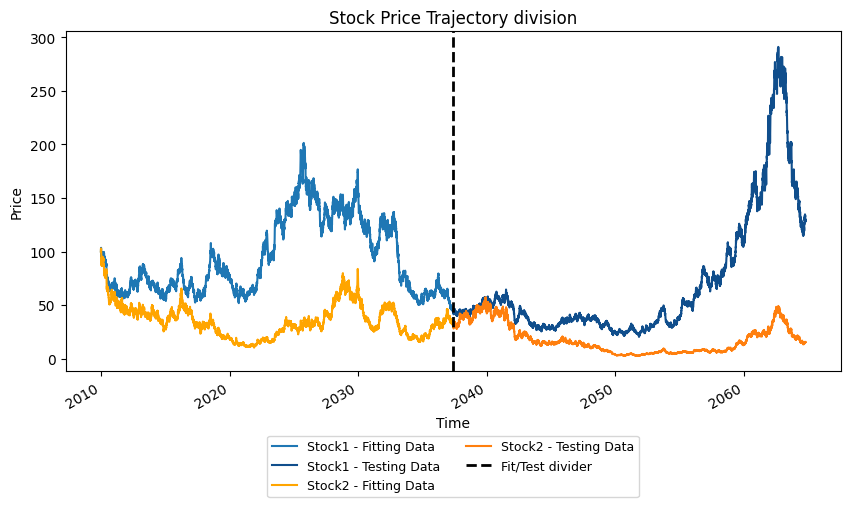
\includegraphics[width=0.8\textwidth]{4Method/pictures/DataDivision.png}
%     \caption{Illustration of how the data is divided into fitting and testing parts. }
%     \label{fig:DataDivision}
% \end{figure}

% \begin{figure}
%     \centering
%     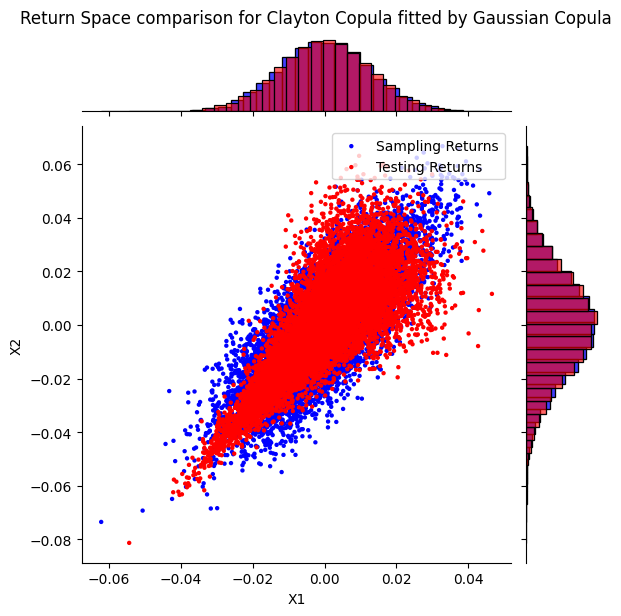
\includegraphics[width=0.5\textwidth]{4Method/pictures/TestSampleComparison.png}
%     \caption{Figure illustrating the difference between the test data and the data sampled from the fitted copula. }
%     \label{fig:TestSampleComparison}
% \end{figure}

% To evaluate the various copulas' ability to accurately capture the dependence between random variables, it is therefore sensible to compare the generated data to the testing data. The reason for using simulated data in this experiment is to ensure that the joint distribution is constant over time as this is a key assumption when using \gls{MC} methods. If the data generated from the fitted copula is similar to the testing data, it shows that the dependence is appropriately modeled by the copula. If not, it shows that the copula is not well suited to model the dependence. Hence this is a good way to evaluate the copulas' performance in an isolated manner. 

% To emphasize the key assumption when using copulas to simulate data for Monte Carlo purposes is that the joint distribution observed in the past continues to be the distribution from which the data is generated into the future. 

% To quantify how similar the test and sampled datasets are to each other, the distance measure described in \Cref{sec:GoodnessOfFit} is used. This allows for computing an average distance that each copula is from the test data over several datasets. This makes it possible to evaluate which copula performs best overall.  


% %%%%%%%%%%%%%%%%%%%%%%%%%%%%%%%%%%%%%%%%%%%%%%%%%%%%%%%%%%%%%%%%%%%%%%%%%%%%%
% %%%% Marginal model test
% %%%%%%%%%%%%%%%%%%%%%%%%%%%%%%%%%%%%%%%%%%%%%%%%%%%%%%%%%%%%%%%%%%%%%%%%%%%%%
% \subsection{Marginal model test}
% To validate that the marginal model works as intended, a test is performed to see how well the fitted marginal distribution matches the true distribution of the data. This is done by generating data from a known distribution and then fitting a marginal model to it. The fitted marginal model is then compared to the true distribution of the data by transforming the data to probability space using the \gls{PIT} using both the fitted distribution and the true distribution. To evaluate how similar the points in probability space are to each other the \gls{MAE} is calculated. Additionally a QQ-plot is created to visualize how well the fitted distribution matches how well the data follows the true distribution. During this experiment it is important to keep in mind that the generated data is subject to random noise, therefore it is not necessarily the case that the true distribution of the data is the exact same as the observed distribution even tough they should be. It is however a good benchmark to see how well the fitted distribution matches the true distribution, which would be a reasonable choice of distribution to use if the neural network was not used. The distributions used for the test are listed in \Cref{tab:distributions} where the distribution, the parameter values, and a short description is displayed for each of the tested distributions. In this test the different terms of the loss function defined in \Cref{sec:NeuralCopulaLoss} are equally weighted. The number of data points used for each distribution is 10000.

% \begin{table}[h]
%     \centering
%     \caption{Distributions and parameters used for the marginal model test.}
%     \begin{tabular}{@{}ccl@{}}
%         Distribution & Parameters & Description \\
%         \toprule
%         Gaussian & $\mu=0, \sigma=1$ & Standard normal distribution \\ 
%         Student's $t$ & $\nu=5$ & Student's $t$-distribution with 5 degrees of freedom \\ 
%         Uniform & $a=0, b=1$ & Uniform distribution on [0, 1] \\ 
%         Exponential & $\lambda=1$ & Exponential distribution with rate 1 \\ 
%         Laplace & $\mu=0, b=1$ & Laplace distribution with mean 0 and scale 1 \\ 
%         Log-normal & $\mu=0, \sigma^2=1$ & Log-normal distribution with mean 0 and variance 1 \\ 
%     \end{tabular}
%     \label{tab:distributions}
% \end{table}



% %%%%%%%%%%%%%%%%%%%%%%%%%%%%%%%%%%%%%%%%%%%%%%%%%%%%%%%%%%%%%%%%%%%%%%%%%%%%%
% %%%% Neural copula testing 
% %%%%%%%%%%%%%%%%%%%%%%%%%%%%%%%%%%%%%%%%%%%%%%%%%%%%%%%%%%%%%%%%%%%%%%%%%%%%%
% \subsection{Neural Copula training scheme test}
% In this section the procedure for finding the best hyper parameters for the model to create a valid copula function is described. Wether or not a copula function is valid is determined by wether or not it satisfies the conditions of being a copula defined in \Cref{def:copula}. In practice for the neural copula this means that all but the first of the loss terms, defined in \Cref{sec:NeuralCopulaLoss}, should approach zero when training is done. Several different combinations of hyper parameters will be tested with the goal of some that work well, meaning that the fitted copula is valid.

% Several datasets will be used for testing the neural copula fitting procedure. This is to ensure that the method works well, regardless of the data, consistently resulting in valid copulas. The method for this workflow is as follows for each dataset. First different datasets will be generated and a grid of different parameter values will be created. The grid will contain different values for the parameters of the neural copula such as the solver used, learning rates, number of epochs, batch size, network architecture and step size scheduler. This creates a large number of different combinations of choices to test which will hopefully result in a method for finding a training method that works well universally. The number of alternatives tested in the grid is somewhat limited to make the execution time reasonable. In total 288\todo{Change} combinations of network parameters are tested for the five datasets. The test will be ran on a compute cluster but despite that the execution time will be long due to the large number of combinations. 

% The datasets that will be used for testing the neural copula fitting procedure are displayed in \Cref{tab:DatasetsTestedOn}. In the table the copula used to generate each dataset is stated along with parameter values. Additionally, the name of the dataset is stated for future reference. The hyper parameters that will be tested are displayed in \Cref{tab:se_hyperparams}. In the table we can see the hyper parameters Network layers and Network neurons that describe the architecture of the \gls{NN}. The parameters Learning rate, Scheduler and Solver describe the training procedure. The parameters Epochs and Batch size describe the training process. 

% \begin{table}[h!]
%     \centering
%     \caption{Datasets used to test the neural copula hyper parameters and loss function weights.}
%     \begin{tabular}{lll}
%     \textbf{Copula} & \textbf{Parameter} & \textbf{Name}  \\
%     \hline
%     Gaussian & $\rho:0$ & Independece \\
%     Gaussian & $\rho:0.7$ & Positive Dependece \\
%     Gaussian & $\rho:-0.7$ & Negative Dependece  \\
%     Gaussian & $\rho:0.999$ & Frechet Upper \\
%     Gaussian & $\rho:-0.999$ & Frechet Lower \\
%     \end{tabular}
%     \label{tab:DatasetsTestedOn}
% \end{table}

% \begin{table}[h!]
%     \centering
%     \caption{Hyperparameter grid choices the test of the neural copula fitting procedure.}
%     \begin{tabular}{ll}
%     \textbf{Hyperparameter} & \textbf{Options} \\
%     \hline
%     Network layers & 2, 3, 4 \\
%     Network neurons & 5, 10 \\
%     Learning rate & 0.1, 0.01 \\
%     Scheduler & step, exponential, None \\
%     Solver & ADAM, SGD \\
%     Epochs & 10000, 5000 \\
%     Batch size & 1024, 2048 (Remove batch size) \\
%     \end{tabular}
%     \label{tab:se_hyperparams}
% \end{table}\todo{Explain some options more}
    

% % For each of the combinations in the grid the an ensemble of runs will be performed to mitigate the impact of what random seeds are used for initializing the weights of the network. The ensemble will consist of 10 runs for each combination in the grid. The best run from the ensemble will be kept for each combination in the grid. 

% The different combinations of hyper parameters will be tested on each of the different datasets. After training the best overall method over the datasets, measured by the average loss, will be selected as the best one. If the losses relating to the copula function constraints close to zero. This indicates that the fitted copula is valid. The best model will be used in the final experiment, described in \Cref{sec:PortfolioTesting}.  

% As a further test, different weights will be used for the different terms in the loss function during training. This is to see what how big the different terms in the loss function should be in relation to each other. We fix the first term to be one, then 0.5, 1, and 2 is tested for the other terms. This test will be conducted using the best performing hyper parameters from the prior part of the test. The evaluation of this test will be done by looking at the equally weighted loss to make the comparison fair. This test is performed for each of the copulas used in the hyper parameter test. The idea of this test is to see if it can be beneficial to weight the different terms in the loss function differently in relation to each other to emphasize some terms in the loss function more. 

% % \begin{generalinstructions}
% % Given generated datasets and a specified grid\\
% % \textbf{For each dataset}
% % \begin{compactitem}
% %     \item \textbf{For grid alternative}
% %     \begin{compactitem}
% %             \item Train copula on dataset
% %         \end{compactitem}
% % \end{compactitem}
% % \textbf{Evaluate the average performance of methods over the datasets}
% % \end{generalinstructions}
 
% \todo{How have i changed the neural copula approach, errors in the neural copula article.}


% %%%%%%%%%%%%%%%%%%%%%%%%%%%%%%%%%%%%%%%%%%%%%%%%%%%%%%%%%%%%%%%%%%%%%%%%%%%%%%
% %%%% Portfolio testing
% %%%%%%%%%%%%%%%%%%%%%%%%%%%%%%%%%%%%%%%%%%%%%%%%%%%%%%%%%%%%%%%%%%%%%%%%%%%%%%
% \subsection{Portfolio testing}\label{sec:PortfolioTesting}
% This section details the steps in the test of the copulas on the different portfolios. 

% \subsubsection{Data Generation}
% To evaluate the performance of different copulas when fitted to data we need data to test the copulas on. The data comes in the form of test portfolios of artificially generated stock price data given that this thesis focuses on the use of copulas in modelling financial returns. These portfolios should ideally cover a wide range of dependence structure types. This is to test the different copulas' versatility and robustness under varying conditions. 

% This thesis focuses on the role of the copula purely and therefore, the aim is not to conflate the results from the copula's performance with that of the marginal fitting procedure. Therefore, we want each marginal distribution of the generated portfolios to be the same known distribution, removing the need for fitting the marginal distributions. The marginal distributions used should not matter, given that the copula is invariant to strictly increasing transformations as stated in \Cref{the:TranslationInvariance}. In this study the marginal distributions used will be the normal distribution. If having different marginal distributions the number of combinations to test during model fitting becomes large. 

% To generate portfolios with different dependence structures and the same marginal distributions, copulas will be used. This will be done by first sampling data from analytical copulas with different parameter values. The result will be data points in probability space that contain the pure dependence between the different variables. These data points will then be plugged into the inverse \gls{CDF} of a Standard normal distribution. This performs the \gls{PIT} in reverse, creating data points with standard normal marginal distributions with the dependence described by the copula. 

% After having generated these pairs of dependent standard, normally distributed random numbers, they are used as the random shocks when simulating the bivariate \gls{GBM} using the Euler-Maruyama scheme defined in \Cref{sec:EulerMaruyama}. This results in test portfolios representing stock prices over time, creating a realistic setting for when using copulas is appropriate. 

% The above procedure for generating data is used for the copulas specified in \Cref{tab:DatasetsUsed}. In the table we can see the different copulas and the parameter values for them. The stock trajectories are simulated for 10000 time periods representing days. Both stocks have a drift term of 0.03 and the volatility is set to 0.2 and 0.3 for stock one and two respectively. 
% \begin{table}[h!]
%     \centering
%     \caption{Portfolios used to evaluate the different copulas.}
%     \begin{tabular}{ll}
%     \textbf{Copula} & \textbf{Parameters} \\
%     \hline
%     Gaussian & Correlation: 0 \\
%     Gaussian & Correlation: 0.7\\
%     Students $t$ & $\rho$: -0.8, $\nu$: 3\\
%     Clayton & Alpha: 4 \\
%     \end{tabular}
%     \label{tab:DatasetsUsed}
% \end{table}

% The resulting portfolios can be observed in \Cref{fig:DatasetsUsed} where the left pictures show the price time series of the different portfolios and the right pictures show the log returns of the portfolios. In the left pictures we can see how the portfolios are divided over time. In the right pictures we can see the log returns of the portfolios. The blue points show the log returns of the fitting data and the red points show the log returns of the testing data. The fitting part will be used in the model fitting and can be thought of as historically observed data. The testing part will be used in the model evaluation and can be thought of as data that will appear in the future, which we want to replicate as well as possible by sampling from a copula fitted to the historical data. 

% \begin{figure}
%     \centering
%     % --- (a) Independence ---
%     \begin{minipage}{0.9\textwidth}
%         \centering
%         \begin{minipage}{0.54\textwidth}
%             \centering
%             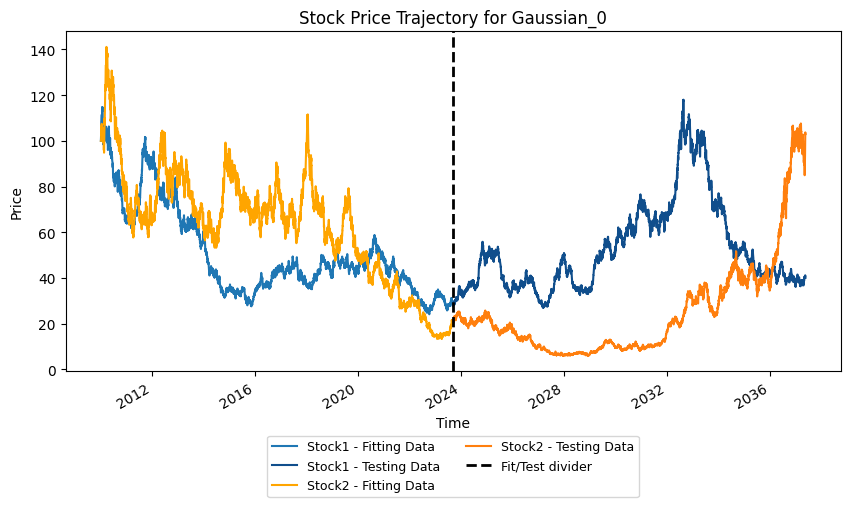
\includegraphics[width=\textwidth]{4Method/pictures/PricesGaussian_0.png}
%             %\subcaption*{Histogram}
%         \end{minipage}
%         \hfill
%         \begin{minipage}{0.34\textwidth}
%             \centering
%             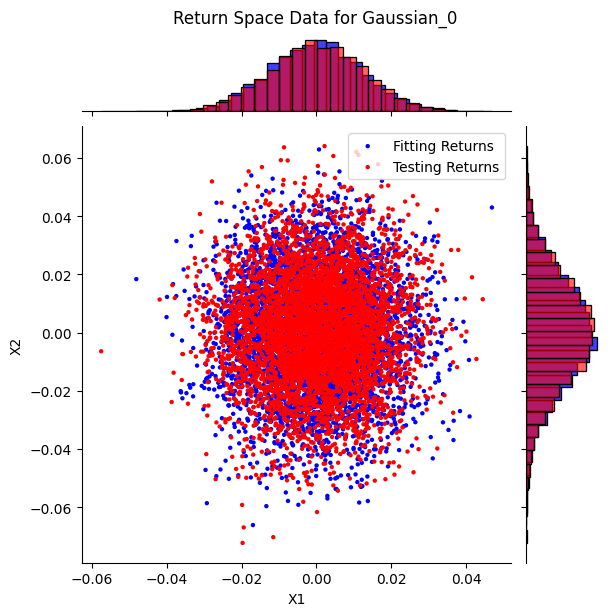
\includegraphics[width=\textwidth]{4Method/pictures/ReturnsGaussian_0.png}
%             %\subcaption*{QQ plot}
%         \end{minipage}
%         \subcaption*{(a) Independent}
%     \end{minipage}
%     \hfill
%     % --- (b) Student's t ---
%     \begin{minipage}{0.9\textwidth}
%         \centering
%         \begin{minipage}{0.54\textwidth}
%             \centering
%             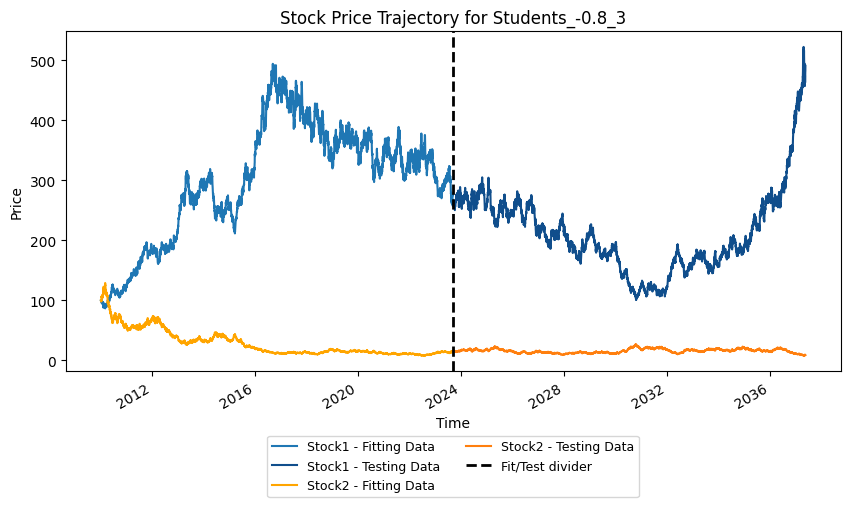
\includegraphics[width=\textwidth]{4Method/pictures/PricesStudents_-08_3.png}
%             %\subcaption*{Histogram}
%         \end{minipage}
%         \hfill
%         \begin{minipage}{0.34\textwidth}
%             \centering
%             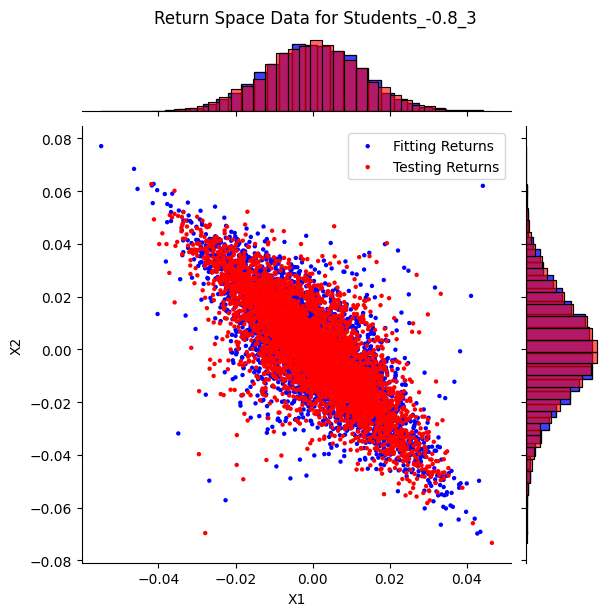
\includegraphics[width=\textwidth]{4Method/pictures/ReturnsStudents_-08_3.png}
%             %\subcaption*{QQ plot}
%         \end{minipage}
%         \subcaption*{(b) Student's $t$ -0.8 3}
%     \end{minipage}
%     \vfill
%     % --- (c) gaussian 0.7 ---
%     \begin{minipage}{0.9\textwidth}
%         \centering
%         \begin{minipage}{0.54\textwidth}
%             \centering
%             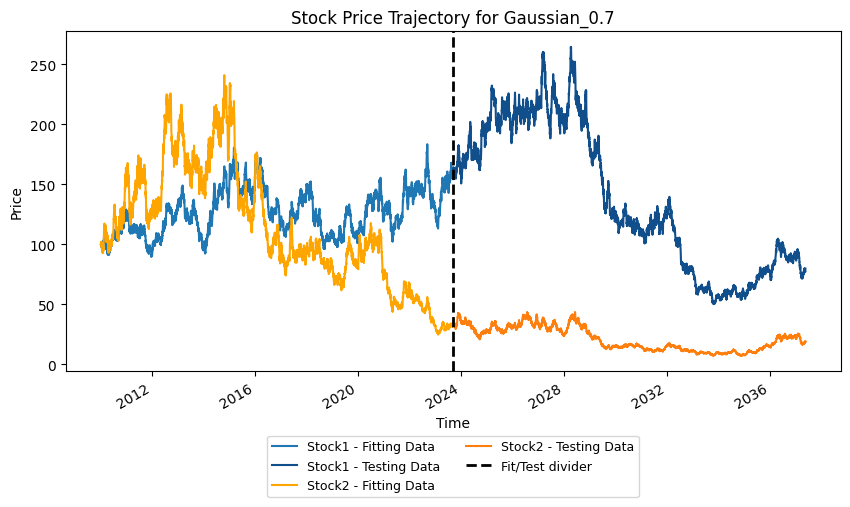
\includegraphics[width=\textwidth]{4Method/pictures/PricesGaussian_07.png}
%             %\subcaption*{Histogram}
%         \end{minipage}
%         \hfill
%         \begin{minipage}{0.34\textwidth}
%             \centering
%             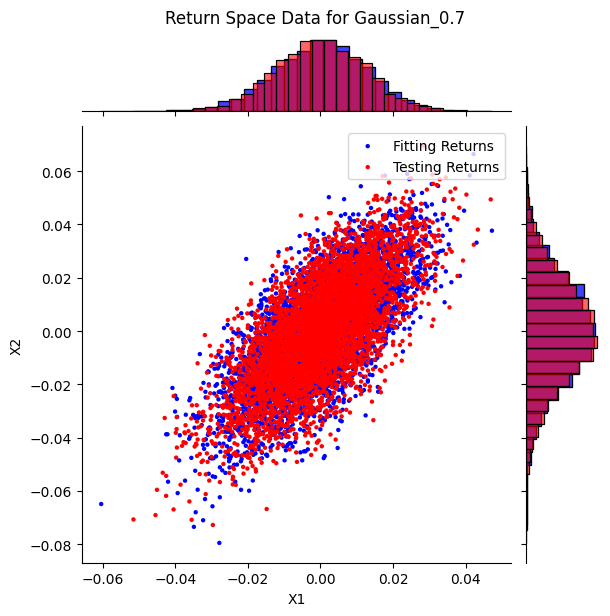
\includegraphics[width=\textwidth]{4Method/pictures/ReturnsGaussian_07.png}
%             %\subcaption*{QQ plot}
%         \end{minipage}
%         \subcaption*{(c) Gaussian 0.7}
%     \end{minipage}
%     \hfill
%     % --- (d) Clayton ---
%     \begin{minipage}{0.9\textwidth}
%         \centering
%         \begin{minipage}{0.54\textwidth}
%             \centering
%             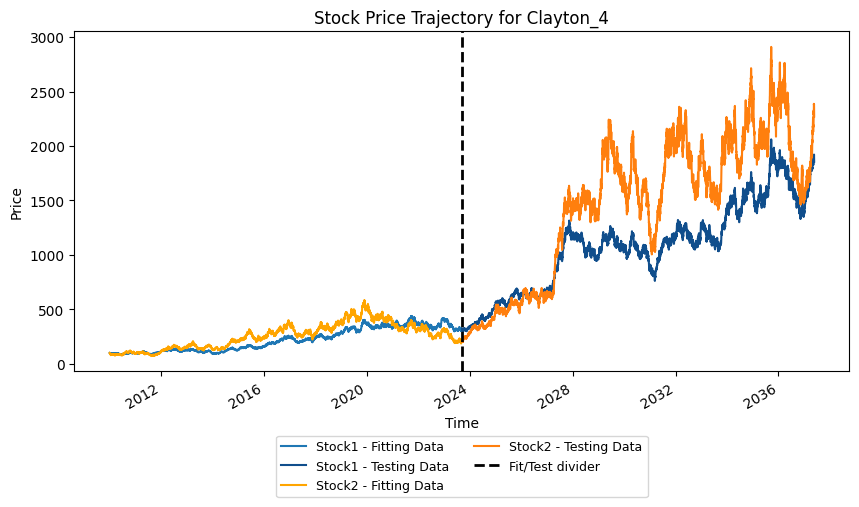
\includegraphics[width=\textwidth]{4Method/pictures/PricesClayton_4.png}
%             %\subcaption*{Histogram}
%         \end{minipage}
%         \hfill
%         \begin{minipage}{0.34\textwidth}
%             \centering
%             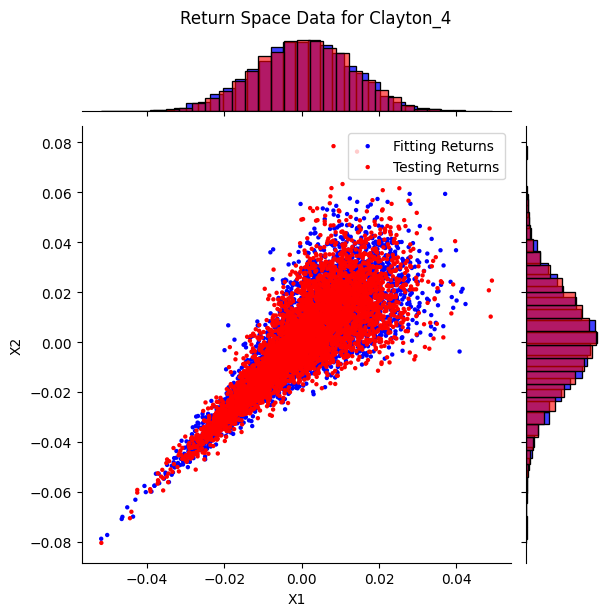
\includegraphics[width=\textwidth]{4Method/pictures/ReturnsClayton_4.png}
%             %\subcaption*{QQ plot}
%         \end{minipage}
%         \subcaption*{(d) Clayton 4}
%     \end{minipage}
%     \caption{Figure displaying the test portfolios price series and log returns for the portfolio test.}
%     \label{fig:DatasetsUsed}
% \end{figure}


% \subsubsection{Model Fitting}
% The fitting data from each of the previously generated portfolios is used for fitting the different copulas. To do this, the data needs to be converted so that the copulas can work with it. Hence, the log returns are calculated as defined in \Cref{def:logReturns}. These are then standardized and centered to have a zero mean and unit variance. 

% The different types of copulas are then fitted as described for the Gaussian in \Cref{sec:GaussianCopula}, the Student's $t$ in \Cref{sec:StudentsCopula}, the Clayton in \Cref{sec:ClaytonCopula} and the \gls{NC} in \Cref{sec:NeuralCopulaFittingAndSampling}. 


% \subsubsection{Model Sampling}
% The main use for copulas is arguably to sample random numbers to be used in \gls{MC} simulations \Citet[p.~40]{Nelsen2006}. The random numbers from the copula can be used to generate dependent realizations of a pair of random variables, regardless of their marginal distributions. Hence, it should make sense to evaluate the copulas based on how well generated random numbers from a fitted copula replicates the true dependence structure of the data. The procedures for sampling from the copulas is described for the Gaussian in \Cref{sec:GaussianCopula}, the Student's $t$ in \Cref{sec:StudentsCopula}, the Clayton in \Cref{sec:ClaytonCopula} and the \gls{NC} in \Cref{sec:NeuralCopulaFittingAndSampling}. 

% The sampled data points from the copulas, other than the \gls{NC} which uses the inverse marginal models, are inserted into the inverse normal distribution and then scaled to match the observed standard deviation of the fitting data. This should generate data similar to the data in the testing part if the copula adequately captures the dependence in the data.

% \subsubsection{Model evaluation}
% To evaluate the performance of each copula for each of the datasets the distance measure described in \Cref{sec:GoodnessOfFit} is used. An average of the distance measure is calculated over the different datasets for each copula. This will give a good indication of how well each copula performs overall. 





% \begin{generalinstructions}
%     \begin{compactenum}
%         \item Data generation
%         \begin{compactenum}
%             \item Generate returns
%             \item Put into GBM as random shocks 
%             \item Calculate log returns 
%             \item Split into different parts (train - test)
%         \end{compactenum}
%         \item Model fitting (for each copula)
%         \item Model evaluation
%         \begin{compactenum}
%             \item Compare the data generated by each copula on distribution level to the testing data for the different datasets
%         \end{compactenum}
%     \end{compactenum}
% \end{generalinstructions}

